\documentclass[american]{scrartcl}
    \usepackage{babel}
    \usepackage[utf8]{inputenc} 
    \usepackage{csquotes}
    \usepackage{amsmath}
    \usepackage{amssymb}
    \usepackage{graphicx}   
    \usepackage{mathtools}
    \usepackage{tikz}

    
    \setlength{\parindent}{0em}
    \setlength{\parskip}{0.5em}

    
    \title{Homework I - Advanced Game Theory }

    % \subtitle{A critical essay on the existing literature}

    \author{Andrea Titton}
    

% Commands
\newcommand{\set}[1]{\left\{#1\right\}}
\newcommand{\Real}{\mathbb{R}}
\newcommand{\abs}[1]{\left\lvert #1 \right\rvert}

% Graphs
\usetikzlibrary{positioning}
\tikzset{main node/.style={circle, draw,minimum size=1cm,inner sep=3pt},}

\begin{document}

% Title

\maketitle

\section*{Exercise 1}

The graph representation of $(N, L)$ is,

\vspace{1cm}
\begin{center}
    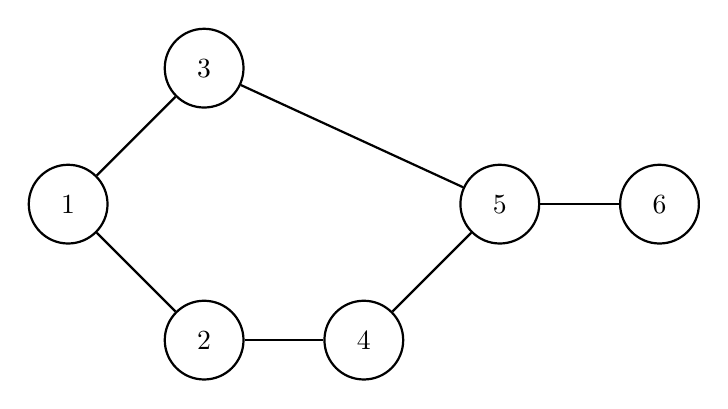
\begin{tikzpicture}[thick]
        % Nodes
        \node[main node] (1) {$1$};
        \node[main node] [below right = 1cm and 1cm of 1] (2) {$2$};
        \node[main node] [above right = 1cm and 1cm of 1] (3) {$3$};
        \node[main node] [right = 1cm of 2] (4) {$4$};
        \node[main node] [above right = 1cm and 1cm of 4] (5) {$5$};
        \node[main node] [right = 1cm of 5] (6) {$6$};
        % Paths
        \path[draw,thick]
        (1) edge node {} (2)
        (1) edge node {} (3)
        (2) edge node {} (4)
        (3) edge node {} (5)
        (4) edge node {} (5)
        (5) edge node {} (6);
    \end{tikzpicture}
\end{center}

\subsection*{(a)}

The function $v^L$ of the Myerson restricted game is,

\begin{equation}
    v^L(S) = \sum_{T \in C_L(S)} v(T).
\end{equation}

It is non-zero only for the component of the graphs that include both $1$ and $6$, namely,

\begin{equation} \label{value_a}
    v^L(S) = \begin{cases}
        1 & \text{ if } S \in \set{\set{1, 3, 5, 6}, \set{1, 2, 3, 5, 6}, \set{1, 2, 4, 5, 6}, \set{1, 3, 4, 5, 6}, \set{1, 2, 3, 4, 5, 6}} \\
        0 & \text{ otherwise }
    \end{cases}
\end{equation}

\subsection*{(b)}

We can define the communication game $(N, v^L)$, using (\ref{value_a}). Then we can compute the Harsanyi dividends based on this game. The non-zero dividends are,

\begin{equation}
    \begin{split}
        \Delta_{v^L}(\set{1, 3, 5, 6}) &= 1 \\
        \Delta_{v^L}(\set{1, 2, 4, 5, 6}) &= 1 \\
        \Delta_{v^L}(\set{1, 2, 3, 4, 5, 6}) &= -1
    \end{split}
\end{equation}

Then we can compute the Myerson value as the Shapley value of the new coordination game,

\begin{equation} \label{myerson_complete}
    \begin{split}
        \mu_i(v, L) = f_i^S &= \sum_{T \in N(i)} \Delta_{v^L}(T) / \abs{T} \\
        \implies \mu(v, L) = f^S &= \begin{pmatrix}
            17/60 & 1/30 & 1/12 & 1/30 & 17/60 & 17/60
        \end{pmatrix}
    \end{split}
\end{equation}

\subsection*{(c)}

The new supply chain is represented by the graph,

\vspace{1cm}
\begin{center}
    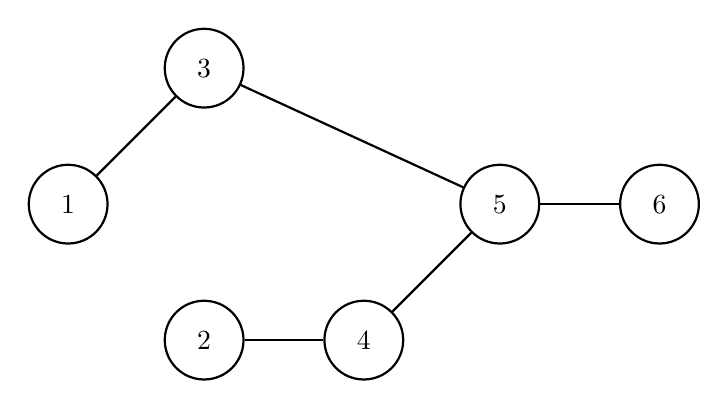
\begin{tikzpicture}[thick]
        % Nodes
        \node[main node] (1) {$1$};
        \node[main node] [below right = 1cm and 1cm of 1] (2) {$2$};
        \node[main node] [above right = 1cm and 1cm of 1] (3) {$3$};
        \node[main node] [right = 1cm of 2] (4) {$4$};
        \node[main node] [above right = 1cm and 1cm of 4] (5) {$5$};
        \node[main node] [right = 1cm of 5] (6) {$6$};
        % Paths
        \path[draw,thick]
        (1) edge node {} (3)
        (2) edge node {} (4)
        (3) edge node {} (5)
        (4) edge node {} (5)
        (5) edge node {} (6);
    \end{tikzpicture}
\end{center}

We can hence define

\begin{equation}
    v^{L^\prime}(S) = \begin{cases}
        0   & \text{ if } S = \set{1, 2, 4, 5, 6} \\
        v^L & \text{ otherwise }
    \end{cases}
\end{equation}

By repeating the procedure of (\ref{myerson_complete}), we obtain,

\begin{equation}
    \mu(v, L^\prime) = \begin{pmatrix}
        1/4 & 0 & 1/4 & 0 & 1/4 & 1/4
    \end{pmatrix}.
\end{equation}

This result is expected since in the new supply chain $2$ and $4$ become null-players.

In order to determine fairness we can check that,

\begin{equation}
    \begin{split}
        \mu_1(v, L) - \mu_1(v, L^\prime) &= \mu_2(v, L) - \mu_2(v, L^\prime) \\
        17/60 - 1 / 4 &= 1/30 - 0 \implies \text{ the fairness axiom is respected.}
    \end{split}
\end{equation}

\subsection*{(d)}

In order to compute the hierarchical outcome of node $1$ we need to set $1$ as root. The resulting directed graph $(N, L^1)$ can be represented as,


\vspace{1cm}
\begin{center}
    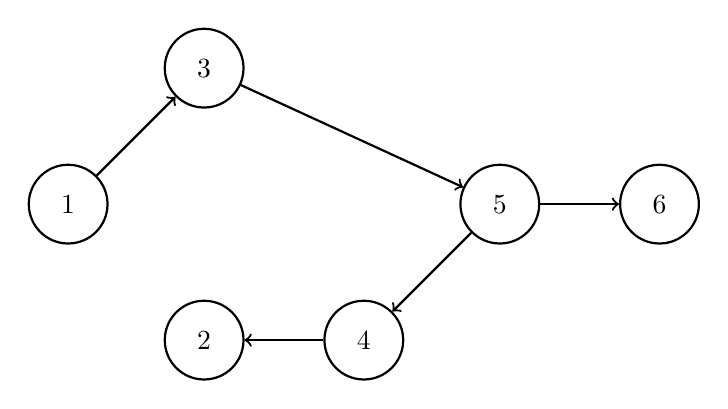
\begin{tikzpicture}[->, thick]
        % Nodes
        \node[main node] (1) {$1$};
        \node[main node] [below right = 1cm and 1cm of 1] (2) {$2$};
        \node[main node] [above right = 1cm and 1cm of 1] (3) {$3$};
        \node[main node] [right = 1cm of 2] (4) {$4$};
        \node[main node] [above right = 1cm and 1cm of 4] (5) {$5$};
        \node[main node] [right = 1cm of 5] (6) {$6$};
        % Paths
        \path[draw,thick]
        (1) edge node {} (3)
        (4) edge node {} (2)
        (3) edge node {} (5)
        (5) edge node {} (4)
        (5) edge node {} (6);
    \end{tikzpicture}
\end{center}

Using the definition of followers and subordinates, we can compute the hierarchical outcomes as,

\begin{equation}
    h^1(v, L^\prime) = \begin{pmatrix}
        v^{L^\prime}(\set{1, 3, 5, 6, 4, 2}) - v^{L^\prime}(\set{3, 5, 6, 4, 2})          \\
        v^{L^\prime}(\set{2})                                                             \\
        v^{L^\prime}(\set{3, 5, 6, 4, 2}) - v^{L^\prime}(\set{5, 6, 4, 2})                \\
        v^{L^\prime}(\set{4, 2}) - v(\set{2})                                             \\
        v^{L^\prime}(\set{5, 6, 4, 2}) - v^{L^\prime}(\set{4, 2}) - v^{L^\prime}(\set{6}) \\
        v^{L^\prime}(6)                                                                   \\
    \end{pmatrix} = \begin{pmatrix}
        1 \\ 0 \\ 0 \\ 0 \\ 0 \\ 0
    \end{pmatrix}
\end{equation}

In a similar manner,

\begin{equation}
    h^4(v, L^\prime) = \begin{pmatrix}
        0 \\ 0 \\ 0 \\ 0 \\ 1 \\ 0
    \end{pmatrix}, \hspace{0.25cm}
    h^6(v, L^\prime) = \begin{pmatrix}
        0 \\ 0 \\ 0 \\ 0 \\ 0 \\ 1
    \end{pmatrix}
\end{equation}

\subsection*{(e)}

The link game $(L^\prime, r^{L^\prime})$ is given by the characteristic function,

\begin{equation} \label{value_r}
    \begin{split}
        \bar{E} &=
        \begin{dcases}
            \begin{rcases}
                \set{(1, 3), (3, 5), (5, 6)} \\
                \set{(1, 3), (4, 2), (3, 5), (5, 6)} \\
                \set{(1, 3), (3, 5), (5, 4), (5, 6)} \\
                \set{(1, 3), (4, 2), (3, 5), (5, 4), (5, 6)}
            \end{rcases}
        \end{dcases}\\
        r^{L^\prime}(E) &= \begin{cases}
            1 & \text{ if } E \in \bar{E} \\
            0 & \text{ otherwise }
        \end{cases}
    \end{split}
\end{equation}


The Shapley value of the link game is,

\begin{equation}
    f^{S}(L^\prime, r^{L^\prime}) = \begin{pmatrix}
        1/3 &
        0   &
        1/3 &
        0   &
        1/3
    \end{pmatrix}
\end{equation}


The associated position value is.

\begin{equation}
    \pi(v, L^\prime) = \begin{pmatrix}
        1/6 &
        0   &
        1/3 &
        0   &
        1/3 &
        1/6
    \end{pmatrix}
\end{equation}

\section*{Exercise 2}

A hierarchical outcome $h^i$ is in the $Core(N, v_L)$ if and only if,

\begin{equation*}
    \sum_{j \in S} h^i_j \geq v(S) \ \text{  and  } \
    \sum_{j \in N} h^i_j = v(N).
\end{equation*}

First let the subordinates of $j$ be

\begin{equation}
    S^i_{j} \coloneqq \set{h: \ \exists (i_1, \dots, i_t) \ s.t. i_1 = j \land i_t = h \land (i_k, i_{k+1}) \in L^i \ \forall  \ k \in \set{1, \dots, t}}
\end{equation}

Entry $j$ in the hierarchical outcome can be written as,

\begin{equation} \label{hier_def}
    h^i_{j} = v(\hat{F}^i_j) - \sum_{h \in F^i_j}  v(\hat{F}^i_h).
\end{equation}

By superadditivity,

\begin{equation}
    \hat{F}^i_j = \set{j} \cup S^i_{j} \implies v(\hat{F}^i_j ) \geq v(j) + v(S^i_{j}).
\end{equation}

Furthermore,

\begin{equation}
    \hat{F}^i_h \subseteq S^i_{j} \ \forall h \in F^i_j \implies \bigcup_{h \in F^i_j} \hat{F}^i_h \subseteq S^i_{j} \implies \sum_{h \in F^i_j}  v(\hat{F}^i_h) \leq v(S^i_{j}).
\end{equation}

Combining these results, we can use (\ref{hier_def}), and show that,

\begin{equation}
    h^i_{j} = v(\hat{F}^i_j) - \sum_{h \in F^i_j}  v(\hat{F}^i_h) \geq v(j) + v(S^i_{j}) - \sum_{h \in F^i_j}  v(\hat{F}^i_h) \geq v(j).
\end{equation}

Given that $h^i_{j} \geq v(j)$, by superadditivity we can show that,

\begin{equation}
    \sum_{j \in S} h^i_{j} \geq \sum_{j \in S} v(j). % TODO: Need to show v(S) \geq \sum v(j)
\end{equation}




\end{document}
